\chapter{Desarrollo del Framework e Integración Modular}
\label{ch:propuesta}

En este capítulo se presenta la arquitectura del framework desarrollado e integrado en este trabajo, denominado \texttt{sarenv-mts}. Se detalla la filosofía de diseño desacoplado del sistema, el flujo de datos entre sus cinco módulos constitutivos y la formulación matemática del middleware de transformación espacial.

\section{Arquitectura General de la Propuesta}

Para conectar de forma robusta la generación de mapas probabilísticos realistas basados en cartografía abierta con los motores de optimización de búsqueda en tiempo mínimo (MTS), se ha diseñado una arquitectura modular basada en cinco bloques funcionales independientes, ilustrada en la Figura~\ref{fig:diagrama_general}.

\begin{figure}[H]
	\ffigbox[\FBwidth]
	{\caption{DIAGRAMA DE ARQUITECTURA GENERAL DEL SISTEMA INTEGRADO SARENV-MTS}}
	{\label{fig:diagrama_general}
	\begin{tikzpicture}[node distance=1.8cm, auto,
	    block/.style={rectangle, draw=azulUC3M, fill=gray97, thick, text width=2.4cm, text centered, rounded corners, minimum height=1.3cm, font=\footnotesize\bfseries},
	    line/.style={draw=azulUC3M, thick, -latex}]
	    
	    \node [block] (m1) {Módulo 1\\Modelado Topológico\\(SAREnv \& LPB)};
	    \node [block, right of=m1, node distance=3.2cm] (m2) {Módulo 2\\Filtro de Restricciones\\(Sindex R-Tree)};
	    \node [block, right of=m2, node distance=3.2cm] (m3) {Módulo 3\\Middleware UTM\\(Proyección X,Y)};
	    \node [block, right of=m3, node distance=3.2cm] (m4) {Módulo 4\\Planificación MTS\\(ACO, ABC, BHA)};
	    \node [block, right of=m4, node distance=3.2cm] (m5) {Módulo 5\\Evaluador SAR\\(PathEvaluator)};
	    
	    \path [line] (m1) -- node[above, font=\tiny] {$POA_{\text{base}}$} (m2);
	    \path [line] (m2) -- node[above, font=\tiny] {$b(v^0)$} (m3);
	    \path [line] (m3) -- node[above, font=\tiny] {JSON / NPY} (m4);
	    \path [line] (m4) -- node[above, font=\tiny] {Trayectorias} (m5);
	\end{tikzpicture}}
\end{figure}

El diseño desacoplado garantiza que cada módulo opere como una pasarela independiente:
\begin{itemize}
    \item El modelado geográfico y probabilístico se calcula una sola vez de forma analítica en el Módulo 1.
    \item El enmascaramiento físico de seguridad y no transitabilidad se ejecuta en el Módulo 2.
    \item El Módulo 3 transforma las coordenadas globales en formato estándar JSON/Numpy compatible con el planificador.
    \item El Módulo 4 ejecuta la optimización bioinspirada de vuelo.
    \item El Módulo 5 realiza el análisis cuantitativo unificado de métricas SAR.
\end{itemize}

\section{Módulo 1: Generación de Cartografía y Probabilidad Espacial}

El primer módulo se encarga de descargar la geometría vectorial de OpenStreetMap y combinarla con el modelo probabilístico \textit{Lost Person Behavior} (LPB) de Robert Koester \cite{koester2008lost}.

\begin{figure}[H]
	\ffigbox[\FBwidth]
	{\caption{FLUJO DEL MÓDULO 1: GENERACIÓN DE PROBABILIDAD TOPOLÓGICA}}
	{\label{fig:diagrama_modulo1}
	\begin{tikzpicture}[node distance=1.5cm, auto,
	    block/.style={rectangle, draw=azulUC3M, fill=gray97, text width=3.8cm, text centered, rounded corners, minimum height=0.9cm, font=\footnotesize},
	    line/.style={draw=azulUC3M, thick, -latex}]
	    
	    \node [block] (osm) {Geometrías OSM (Casa de Campo)};
	    \node [block, below of=osm] (lpb) {Pesos Estadísticos por Perfil LPB};
	    \node [block, below of=lpb] (dist) {Dispersión Radial Log-Normal (LKP)};
	    \node [block, right of=lpb, node distance=5.5cm] (fusion) {\textbf{Suma Ponderada y Normalización}\\$\mathbf{POA}(i,j) = \frac{\sum_k \mathbf{M}_k \alpha_k}{\sum \mathbf{POA}}$};
	    \node [block, right of=fusion, node distance=4.5cm] (out1) {Matriz Base (.npy)};
	    
	    \path [line] (osm) -| (fusion);
	    \path [line] (lpb) -- (fusion);
	    \path [line] (dist) -| (fusion);
	    \path [line] (fusion) -- (out1);
	\end{tikzpicture}}
\end{figure}

Como se describió en el Capítulo 3, las capas semánticas (caminos, bosques, estructuras, agua, prados) se rasterizan en matrices binarias $\mathbf{M}_k$ y se combinan mediante una suma ponderada lineal, preservando los picos de verosimilitud de las intersecciones lineales.

\section{Módulo 2: Motor de Filtrado de Restricciones Físicas (\texttt{Sindex})}

El segundo módulo proyecta las geometrías de exclusión física (lagos profundos y edificaciones cerradas) sobre la rejilla espacial utilizando árboles de indexación jerárquica R-Tree (\texttt{sindex}), como se sintetiza en la Figura~\ref{fig:diagrama_modulo2}.

\begin{figure}[H]
	\ffigbox[\FBwidth]
	{\caption{FLUJO DEL MÓDULO 2: FILTRADO ESPACIAL DE RESTRICCIONES DURAS}}
	{\label{fig:diagrama_modulo2}
	\begin{tikzpicture}[node distance=1.5cm, auto,
	    block/.style={rectangle, draw=azulUC3M, fill=gray97, text width=3.8cm, text centered, rounded corners, minimum height=0.9cm, font=\footnotesize},
	    line/.style={draw=azulUC3M, thick, -latex}]
	    
	    \node [block] (in) {Matriz Base $\mathbf{POA}_{\text{base}}$};
	    \node [block, below of=in] (polys) {Polígonos No Transitables (Agua / Edificios)};
	    \node [block, right of=in, node distance=5.5cm] (mask) {\textbf{Máscara Espacial R-Tree}\\Anulación Estricta: $P(i,j) = 0.0$};
	    \node [block, below of=mask] (renorm) {Renormalización Global\\$\sum_{i,j} b(v^0)(i,j) = 1.0$};
	    \node [block, right of=mask, node distance=4.5cm] (out2) {Mapa de Creencias $b(v^0)$};
	    
	    \path [line] (in) -- (mask);
	    \path [line] (polys) -| (mask);
	    \path [line] (mask) -- (renorm);
	    \path [line] (renorm) -| (out2);
	\end{tikzpicture}}
\end{figure}

Este paso garantiza que los algoritmos de optimización reciban una distribución de probabilidad depurada $b(v^0)$, eliminando el desperdicio de batería sobre tejados o masas de agua y modelando una búsqueda aérea coordinada.

\section{Módulo 3: Middleware de Transformación de Coordenadas}

El tercer módulo actúa como pasarela matemática entre la cartografía georreferenciada global y la rejilla matricial discreta de simulación de MTS.

\begin{figure}[H]
	\ffigbox[\FBwidth]
	{\caption{FLUJO DEL MÓDULO 3: TRANSFORMACIÓN Y EXPORTACIÓN DEL MIDDLEWARE}}
	{\label{fig:diagrama_modulo3}
	\begin{tikzpicture}[node distance=1.5cm, auto,
	    block/.style={rectangle, draw=azulUC3M, fill=gray97, text width=4.0cm, text centered, rounded corners, minimum height=0.9cm, font=\footnotesize},
	    line/.style={draw=azulUC3M, thick, -latex}]
	    
	    \node [block] (utm) {Coordenadas UTM EPSG:32630\\$(x_{\min}, y_{\min}, x_{\max}, y_{\max})$};
	    \node [block, right of=utm, node distance=5.5cm] (trans) {\textbf{Transformación a Rejilla}\\$X = \lfloor \frac{\Delta x}{\delta} \rfloor, \quad Y = \lfloor \frac{\Delta y}{\delta} \rfloor$\\Resolución: $\delta = 10\text{ m}$};
	    \node [block, right of=trans, node distance=4.8cm] (json) {Escenario JSON / NPY\\Listo para MTS};
	    
	    \path [line] (utm) -- (trans);
	    \path [line] (trans) -- (json);
	\end{tikzpicture}}
\end{figure}

\subsection{Formulación Matemática de la Proyección de Coordenadas}

Sea el Punto de Planificación Inicial o punto de despegue $LKP = (\text{lon}_{\text{LKP}}, \text{lat}_{\text{LKP}})$. El middleware realiza los siguientes pasos:
\begin{enumerate}
    \item \textbf{Proyección Geográfica a UTM:} Se proyecta el par angular $(\text{lon}, \text{lat})$ a coordenadas métricas globales UTM Zona 30 Norte ($\text{EPSG:32630}$):
    \begin{equation}
        (x_{\text{UTM}}, y_{\text{UTM}}) = \mathcal{T}_{\text{WGS84}\to\text{UTM}}(\text{lon}_{\text{LKP}}, \text{lat}_{\text{LKP}})
    \end{equation}
    \item \textbf{Cálculo de Distancias Relativas al Origen del Escenario:} Sabiendo que el origen de la rejilla $(0,0)$ corresponde a la esquina inferior izquierda $(x_{\min}, y_{\min})$:
    \begin{equation}
        \Delta x = x_{\text{UTM}} - x_{\min}, \quad \Delta y = y_{\text{UTM}} - y_{\min}
    \end{equation}
    \item \textbf{Discretización a Índices Matriciales:} Dividiendo por la resolución espacial $\delta = 10\text{ m}$:
    \begin{equation}
        X_{\text{local}} = \left\lfloor \frac{\Delta x}{\delta} \right\rfloor, \quad Y_{\text{local}} = \left\lfloor \frac{\Delta y}{\delta} \right\rfloor
    \end{equation}
\end{enumerate}
El vector resultante $(X_{\text{local}}, Y_{\text{local}})$ define unívocamente la posición de despegue fija en la matriz discreta de MTS.

\subsection{Estructura de Intercambio del Escenario (\texttt{escenario.json})}

Para desacoplar el procesamiento cartográfico de la lógica de optimización, el middleware genera un archivo de configuración estandarizado en formato JSON vinculado a la matriz binaria \texttt{.npy}. Este fichero articula los parámetros cinemáticos, sensoriales y dimensionales de la misión:
\begin{itemize}
    \item \texttt{size}: Dimensiones matriciales de la rejilla $[N_x, N_y]$ ($458 \times 481$ celdas para la Casa de Campo).
    \item \texttt{init\_pos}: Vector de despegue $[[X_{\text{local}}, Y_{\text{local}}]]$ derivado del LKP.
    \item \texttt{posible\_moves}: Conectividad cinemática del UAV, fijada en 8 direcciones contiguas (vecindad de Moore: N, NE, E, SE, S, SW, W, NW).
    \item \texttt{num\_steps}: Presupuesto temporal de vuelo máximo ($T = 1000$ pasos por misión).
    \item \texttt{height} y \texttt{dmax}: Parámetros de altitud de crucero y huella sensorial efectiva ($R_d = 50\text{ m}$).
    \item \texttt{algoritmo\_busqueda}: Planificador seleccionado (\texttt{aco}, \texttt{abc}, \texttt{bha} o baselines de referencia).
\end{itemize}

\section{Módulo 4: Motor de Simulación y Algoritmos Bioinspirados (MTS)}

El Módulo 4 constituye el núcleo de enrutamiento deliberativo del sistema, integrando y extendiendo el framework \textit{MTS-UncertainEnvironment} \cite{Broton_Gutierrez_MTS-UncertainEnvironment}. A partir del mapa de creencias inicial $b(v^0)$ y las restricciones físicas calculadas en los módulos precedentes, el planificador genera trayectorias de vuelo optimizadas para interceptar a la víctima en tiempo mínimo.

\subsection{Formulación del Problema de Optimización de Trayectorias}

Sea $\mathcal{S} \subset \mathbb{Z}^2$ el espacio discreto de celdas de la rejilla y $\mathcal{M}$ el conjunto de movimientos admisibles de 8 conectividad. Una trayectoria para un UAV en un horizonte de tiempo $T$ se define como una secuencia ordenada de posiciones:
\begin{equation}
\pi = \left( p_0, p_1, p_2, \dots, p_T \right), \quad p_t \in \mathcal{S}, \quad p_{t+1} - p_t \in \mathcal{M}
\end{equation}
con $p_0 = (X_{\text{local}}, Y_{\text{local}})$. El objetivo del planificador es encontrar la trayectoria $\pi^*$ que maximice la ganancia acumulada de probabilidad de detección sobre el mapa dinámico de creencias $b(v^t)$ actualizado recursivamente mediante el RBF:
\begin{equation}
\pi^* = \arg\max_{\pi} \sum_{t=0}^{T} \sum_{(x,y) \in \text{FoV}(p_t)} b(v^t)(x, y)
\end{equation}
donde $\text{FoV}(p_t)$ denota el conjunto de celdas contenidas en la huella del sensor circular de radio $R_d = 50\text{ m}$ centrado en la posición $p_t$.

\subsection{Colonia de Hormigas (Ant Colony Optimization - ACO)}

La formulación de ACO en MTS implementa el esquema \textit{Max-Min Ant System} (MMAS) con feromona espacial 2D, adaptando los desarrollos de Carabaza et al. \cite{carabaza-ACOr, carabaza_ingles}:
\begin{enumerate}
    \item \textbf{Construcción Probabilística de Rutas:} Cada hormiga artificial construye una trayectoria desde $p_0$. La probabilidad de transición de la celda actual $i$ a la celda vecina $j \in \mathcal{N}(i)$ se rige por:
    \begin{equation}
    P_{ij} = \frac{[\tau_{ij}]^\alpha \cdot [\eta_{ij}]^\beta}{\sum_{l \in \mathcal{N}(i)} [\tau_{il}]^\alpha \cdot [\eta_{il}]^\beta}
    \end{equation}
    donde $\tau_{ij}$ representa la traza de feromona acumulada en el movimiento $i \to j$, y $\eta_{ij}$ es la deseabilidad heurística local, proporcional a la densidad de creencia $b(v^k)$ observable en el entorno de $j$. Los exponentes $\alpha$ y $\beta$ ponderan la influencia relativa del rastro histórico frente a la ganancia inmediata.
    \item \textbf{Evaporación y Depósito Acotado de Feromona:} Para evitar la convergencia prematura hacia óptimos locales, la feromona se evapora a una tasa $\rho \in (0,1)$, y solo la mejor hormiga global deposita nueva feromona $\Delta \tau$, acotando estrictamente los valores en el intervalo $[\tau_{\min}, \tau_{\max}]$:
    \begin{equation}
    \tau_{ij}(t+1) = \max \left( \tau_{\min}, \min \left( \tau_{\max}, (1-\rho)\tau_{ij}(t) + \Delta \tau_{ij}^{\text{best}} \right) \right)
    \end{equation}
\end{enumerate}

\subsection{Colonia de Abejas Artificiales (Artificial Bee Colony - ABC)}

El algoritmo ABC, adaptado a partir del paradigma original de Karaboga y Basturk \cite{karaboga2007}, modela la optimización de rutas mediante una población de fuentes de alimento (cada una representando una política o secuencia de decisiones de rumbo) gestionada por tres grupos de agentes:
\begin{enumerate}
    \item \textbf{Abejas Empleadas:} Cada abeja empleada está asociada a una trayectoria candidata $\mathbf{x}_i$. En cada iteración, explora las proximidades de su solución aplicando una perturbación estocástica:
    \begin{equation}
    v_{ij} = x_{ij} + \phi_{ij} (x_{ij} - x_{kj}), \quad \phi_{ij} \in [-1, 1]
    \end{equation}
    donde $k$ es otra solución seleccionada al azar. Si la nueva trayectoria produce una mayor absorción bayesiana, reemplaza a la anterior; en caso contrario, se incrementa un contador de estancamiento.
    \item \textbf{Abejas Observadoras:} Evalúan la calidad de todas las fuentes mediante un mecanismo de ruleta probabilística proporcional a su \textit{fitness} $J(\pi_i)$:
    \begin{equation}
    p_i = \frac{J(\pi_i)}{\sum_{m=1}^{SN} J(\pi_m)}
    \end{equation}
    Las observadoras concentran un mayor esfuerzo de refinamiento en las trayectorias que sobrevuelan zonas de alta densidad de personas extraviadas.
    \item \textbf{Abejas Exploradoras:} Si el contador de estancamiento de una fuente supera el umbral prefijado (\texttt{limit}), la solución se descarta por haberse agotado su margen de mejora local, y la abeja se transforma en exploradora, generando una nueva trayectoria en regiones inexploradas para mantener la diversidad del enjambre.
\end{enumerate}

\subsection{Algoritmo de Agujeros Negros (Black Hole Algorithm - BHA)}

Inspirado en la mecánica gravitatoria cósmica formulada por Hatamlou \cite{hatamlou2012}, BHA opera sobre una población de $N_{\text{stars}}$ trayectorias candidatas denominadas estrellas:
\begin{enumerate}
    \item \textbf{Identificación del Agujero Negro:} La trayectoria con mayor valor de absorción de probabilidad acumulada es designada como el Agujero Negro central ($\mathbf{X}_{BH}$).
    \item \textbf{Atracción Gravitacional de Soluciones:} En cada paso del algoritmo, todas las estrellas son atraídas hacia la trayectoria líder modificando sus vectores de decisión:
    \begin{equation}
    \mathbf{X}_i(t+1) = \mathbf{X}_i(t) + \mathbf{r} \cdot \left( \mathbf{X}_{BH} - \mathbf{X}_i(t) \right)
    \end{equation}
    donde $\mathbf{r}$ es un vector aleatorio con distribución uniforme en $[0, 1]$. Si una estrella supera en \textit{fitness} al agujero negro actual, asume inmediatamente el rol de nuevo agujero negro.
    \item \textbf{Horizonte de Sucesos y Regeneración Estocástica:} Para evitar el colapso prematuro de la población en un único punto, se define el radio del horizonte de sucesos (análogo al radio de Schwarzschild):
    \begin{equation}
    R_{EH} = \frac{J(\mathbf{X}_{BH})}{\sum_{i=1}^{N_{\text{stars}}} J(\mathbf{X}_i)}
    \end{equation}
    Cualquier estrella cuya distancia euclídea al agujero negro sea inferior a $R_{EH}$ se considera absorbida, destruida y regenerada aleatoriamente en el espacio de búsqueda.
\end{enumerate}

\subsection{Planificadores Clásicos de Referencia (Baselines)}

Para contrastar el beneficio de los métodos bioinspirados frente a las estrategias estándar de rescate, el Módulo 4 incorpora tres algoritmos clásicos:
\begin{itemize}
    \item \textbf{Búsqueda Voraz (\textit{Greedy}):} En cada celda $p_t$, el UAV evalúa sus 8 vecinos admisibles y avanza hacia aquel con la mayor densidad de creencia $b(v^t)$, sin planificación a largo plazo.
    \item \textbf{Patrón Boustrophedon (\textit{Lawnmower}):} Cobertura geométrica sistemática en pasadas paralelas de ida y vuelta, cubriendo exhaustivamente el terreno sin guiado probabilístico.
    \item \textbf{Espiral Expansiva (\textit{Expanding Spiral}):} Trayectoria geométrica de radios crecientes centrada en el LKP, representativa de las búsquedas visuales manuales en rescate tradicional.
\end{itemize}

\section{Módulo 5: Evaluador Centralizado de Métricas SAR (\texttt{PathEvaluatorTFM})}

El Módulo 5 centraliza la evaluación cuantitativa independiente de todas las trayectorias generadas, aplicando el estándar del módulo \texttt{PathEvaluatorTFM}:

\begin{figure}[H]
	\ffigbox[\FBwidth]
	{\caption{FLUJO DEL MÓDULO 5: EVALUACIÓN UNIFICADA DE RENDIMIENTO SAR}}
	{\label{fig:diagrama_modulo5}
	\begin{tikzpicture}[node distance=1.5cm, auto,
	    block/.style={rectangle, draw=azulUC3M, fill=gray97, text width=3.8cm, text centered, rounded corners, minimum height=0.9cm, font=\footnotesize},
	    line/.style={draw=azulUC3M, thick, -latex}]
	    
	    \node [block] (traj) {Trayectoria $(X,Y)$ y Telemetría CSV};
	    \node [block, below of=traj] (map) {Mapa de Creencias Base $b(v^0)$};
	    \node [block, right of=traj, node distance=5.5cm] (eval) {\textbf{PathEvaluatorTFM}\\Cálculo Vectorial Shapely / RBF};
	    \node [block, right of=eval, node distance=4.5cm] (metrics) {5 Métricas SAR Oficiales (CSV / Boxplots)};
	    
	    \path [line] (traj) -- (eval);
	    \path [line] (map) -| (eval);
	    \path [line] (eval) -- (metrics);
	\end{tikzpicture}}
\end{figure}

Las cinco métricas evaluadas son:
\begin{enumerate}
    \item \textbf{Tasa de Éxito (\textit{Success Rate}, \%):} Porcentaje de misiones en las que el dron intercepta la víctima virtual a una distancia $d \le 50\text{ m}$.
    \item \textbf{Pasos hasta el Hallazgo (\textit{Steps to Goal}):} Número de instantes temporales transcurridos hasta la detección.
    \item \textbf{Probabilidad Acumulada Absorbida (\textit{Reduced Belief}, \%):} Fracción de la masa de probabilidad total del mapa eliminada tras el paso del sensor.
    \item \textbf{Área Geográfica Barrida (\textit{Covered Area}, $\text{km}^2$):} Superficie neta cubierta por la huella del sensor sin duplicar solapamientos.
    \item \textbf{Distancia de Vuelo (\textit{Total Flight Length}, km):} Longitud métrica total de la trayectoria recorrida.
\end{enumerate}

\section{Herramientas de Control y Validación Interactiva (Jupyter Notebooks)}

Para facilitar la experimentación, inspección visual y demostración en tiempo real de los algoritmos, se ha desarrollado un conjunto de cuadernos interactivos en Jupyter (\texttt{Notebook\_Demo\_Rapida\_Interactiva.ipynb}), cuya interfaz dual se ilustra en la Figura~\ref{fig:demo_interactiva}.

\begin{figure}[H]
	\ffigbox[\FBwidth]
	{\caption{PANEL DUAL DE SIMULACIÓN Y MÉTRICAS EN TIEMPO REAL (DEMO INTERACTIVA)}}
	{\label{fig:demo_interactiva}
	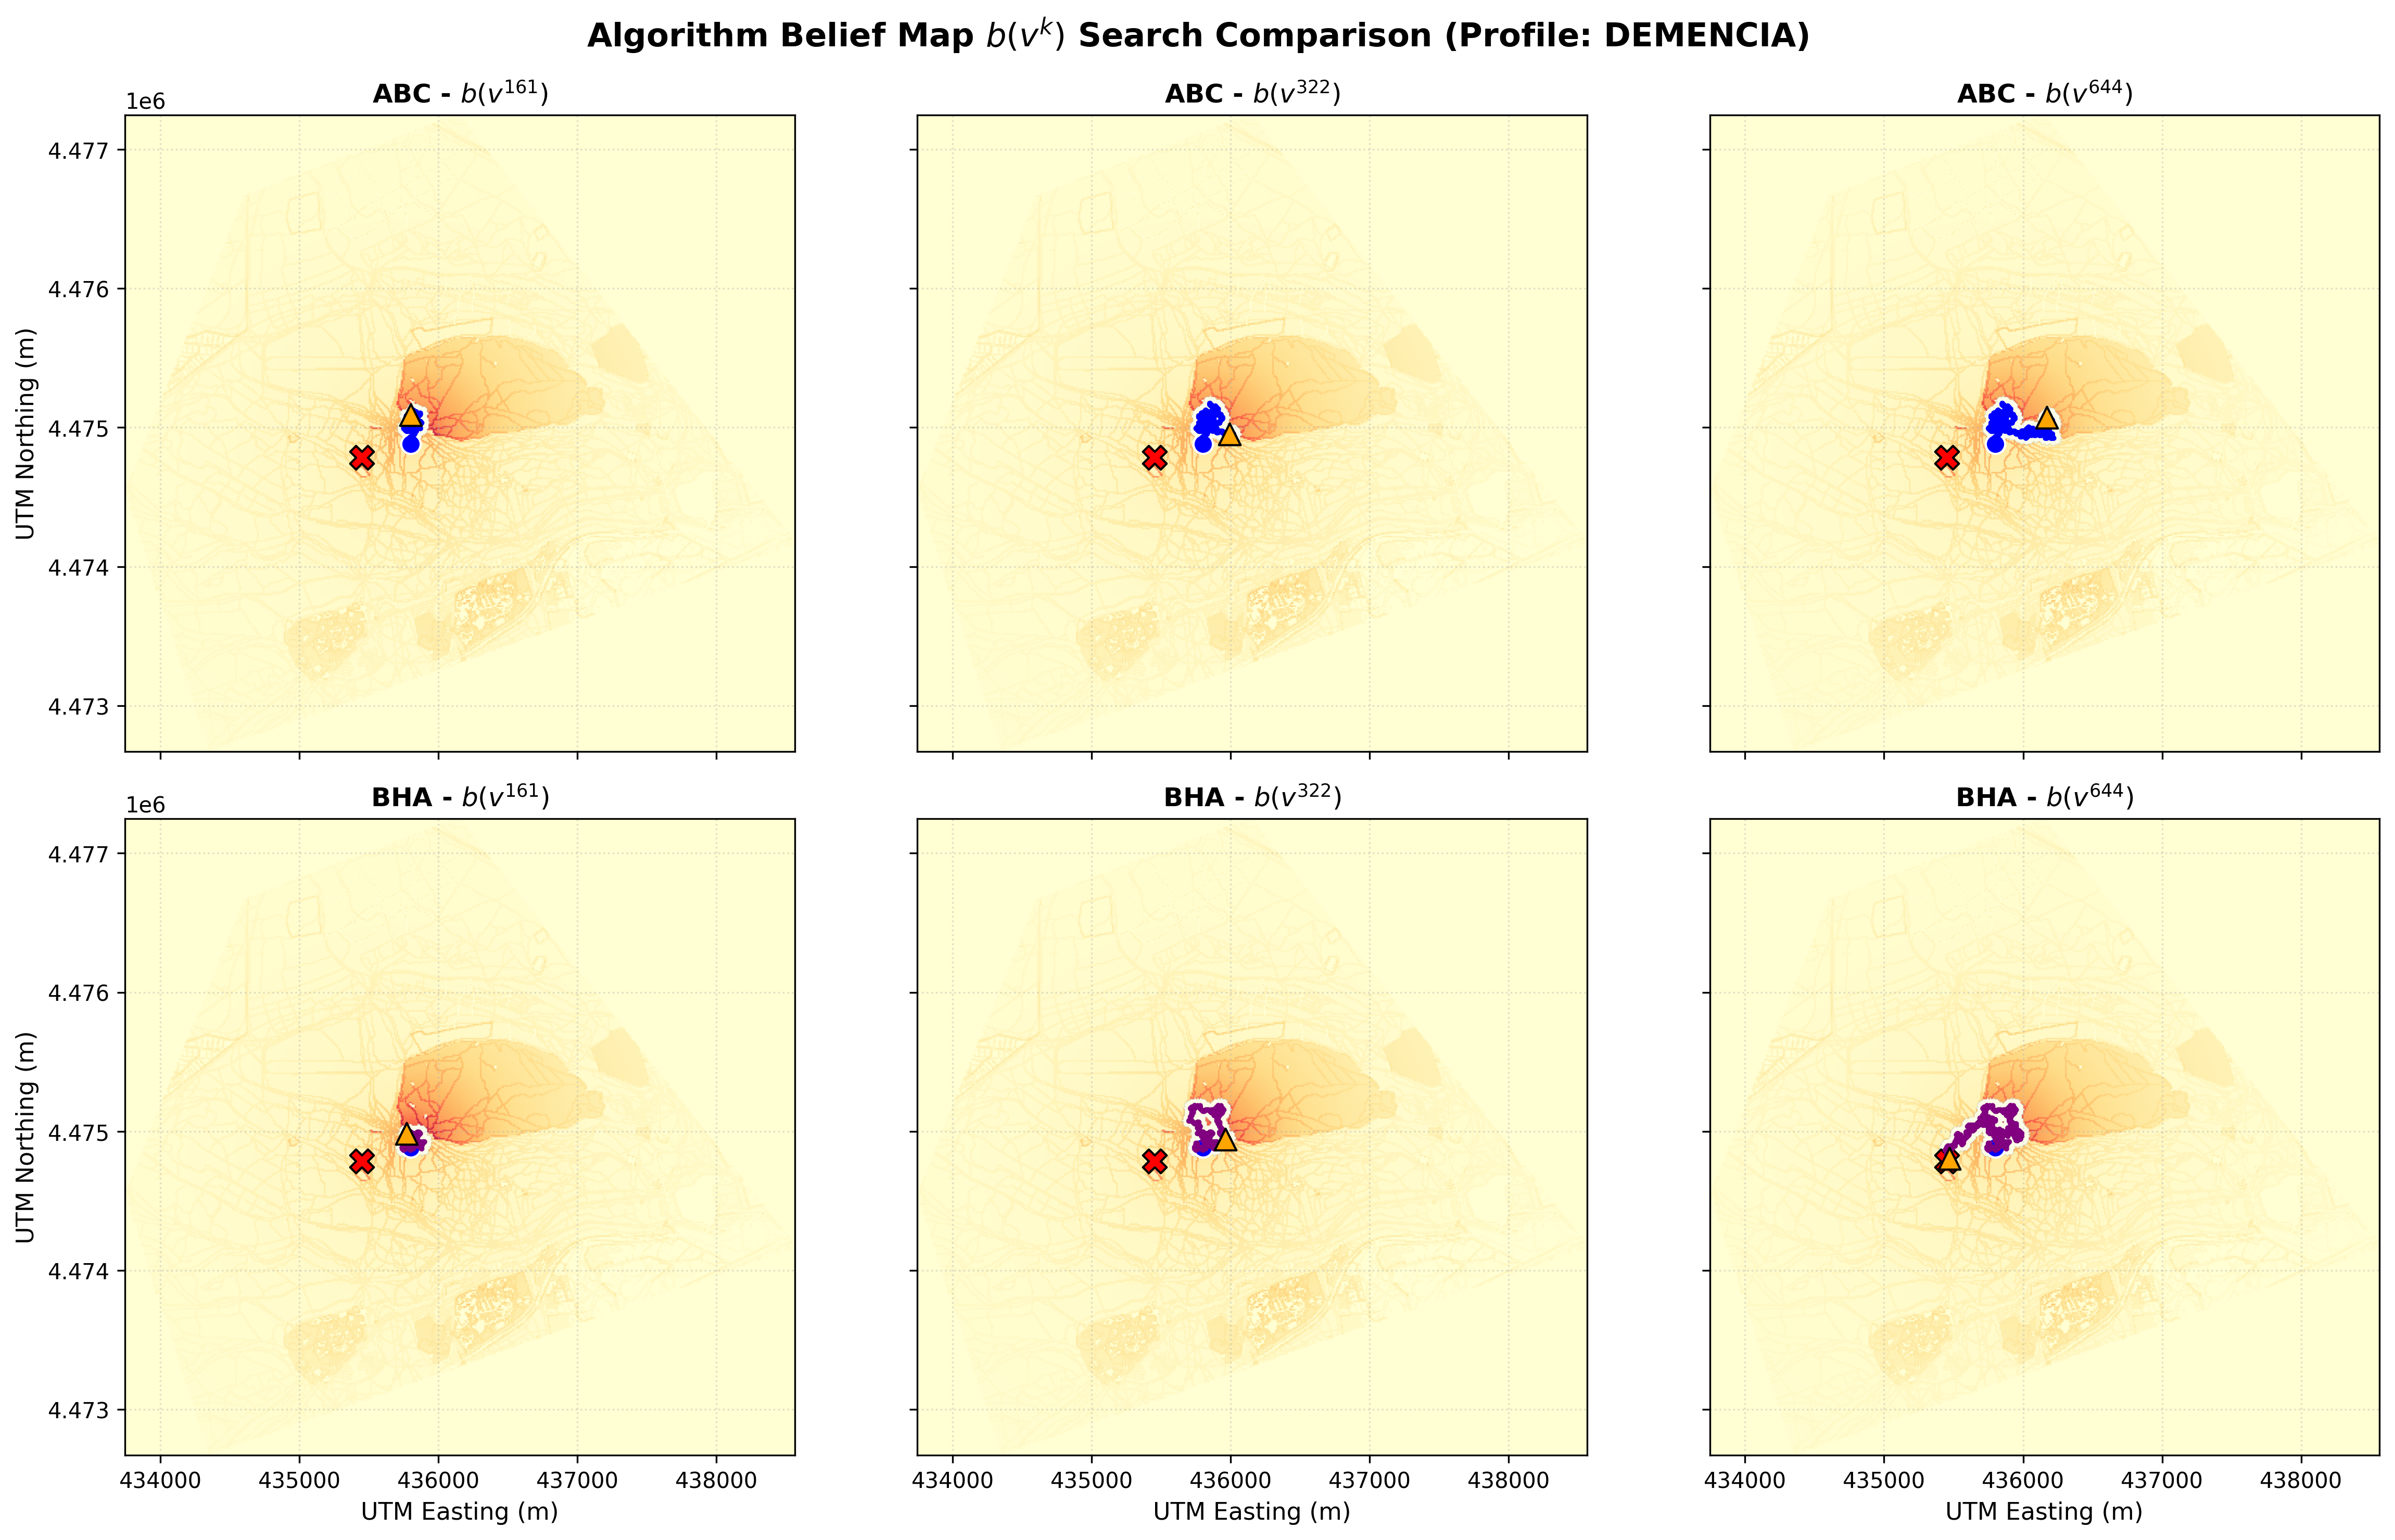
\includegraphics[width=0.95\textwidth]{imagenes/comparativa_evolucion_demencia_abc_vs_bha.png}}
\end{figure}

Esta herramienta permite al operador seleccionar de forma interactiva el perfil de la víctima, visualizar el mapa de calor con restricciones, seleccionar el algoritmo deseado y observar instantáneamente tanto la trayectoria volada como el mapa de creencias residual $b(v^{\text{Final}})$ con su correspondiente cuadro de métricas SAR.
